\documentclass[12pt]{report}
\usepackage[utf8]{inputenc}
\usepackage[russian]{babel}
%\usepackage[14pt]{extsizes}
\usepackage{listings}
\usepackage{graphicx}
\usepackage{amsmath,amsfonts,amssymb,amsthm,mathtools} 
\usepackage{pgfplots}
\usepackage{filecontents}
\usepackage{indentfirst}
\usepackage{eucal}
\usepackage{enumitem}
\frenchspacing

\usepackage{indentfirst} % Красная строка


\usetikzlibrary{datavisualization}
\usetikzlibrary{datavisualization.formats.functions}

\usepackage{amsmath}



% Для листинга кода:
\usepackage{caption}
\DeclareCaptionFont{white}{\color{white}}
\DeclareCaptionFormat{listing}{\colorbox{white}{\parbox{\textwidth}{#1#2#3}}}
\captionsetup[lstlisting]{format=listing,justification=raggedright}

\lstset{ %
	language=python,                 % выбор языка для подсветки
	basicstyle=\small\sffamily, % размер и начертание шрифта для подсветки кода
	keywordstyle=\color{blue},
	numbers=left,               % где поставить нумерацию строк (слева\справа)
	numberstyle=\tiny,           % размер шрифта для номеров строк
	stepnumber=1,                   % размер шага между двумя номерами строк
	numbersep=5pt,                % как далеко отстоят номера строк от подсвечиваемого кода
	showspaces=false,            % показывать или нет пробелы специальными отступами
	showstringspaces=false,      % показывать или нет пробелы в строках
	showtabs=false,             % показывать или нет табуляцию в строках
	frame=single,              % рисовать рамку вокруг кода
	tabsize=2,                 % размер табуляции по умолчанию равен 2 пробелам
	captionpos=t,              % позиция заголовка вверху [t] или внизу [b] 
	breaklines=true,           % автоматически переносить строки (да\нет)
	breakatwhitespace=false, % переносить строки только если есть пробел
	escapeinside={\#*}{*)}   % если нужно добавить комментарии в коде
}

\usepackage[left=2cm,right=2cm, top=2cm,bottom=2cm,bindingoffset=0cm]{geometry}
% Для измененных титулов глав:
\usepackage{titlesec, blindtext, color} % подключаем нужные пакеты
\definecolor{gray75}{gray}{0.75} % определяем цвет
\newcommand{\hsp}{\hspace{20pt}} % длина линии в 20pt
% titleformat определяет стиль
\titleformat{\chapter}[hang]{\Huge\bfseries}{\thechapter\hsp\textcolor{gray75}{|}\hsp}{0pt}{\Huge\bfseries}


% plot
\usepackage{pgfplots}
\usepackage{filecontents}
\usetikzlibrary{datavisualization}
\usetikzlibrary{datavisualization.formats.functions}

\begin{document}
	\def\contentsname{Содержание}
	\def\refname{Список литературы}
	\thispagestyle{empty}
	\begin{titlepage}
		\noindent \begin{minipage}{0.15\textwidth}
			
\includegraphics[width=\linewidth]{b_logo}
		\end{minipage}
		\noindent\begin{minipage}{0.9\textwidth}\centering
			\textbf{Министерство науки и высшего образования Российской Федерации}\\
			\textbf{Федеральное государственное бюджетное образовательное учреждение высшего образования}\\
			\textbf{~~~«Московский государственный технический университет имени Н.Э.~Баумана}\\
			\textbf{(национальный исследовательский университет)»}\\
			\textbf{(МГТУ им. Н.Э.~Баумана)}
		\end{minipage}
		
		\noindent\rule{18cm}{3pt}
		\newline\newline
		\noindent ФАКУЛЬТЕТ $\underline{\text{«Информатика и системы управления»}}$ \newline\newline
		\noindent КАФЕДРА $\underline{\text{«Программное обеспечение ЭВМ и информационные технологии»}}$\newline\newline\newline\newline\newline
		
		
		\begin{center}
			\noindent\begin{minipage}{1.3\textwidth}\centering
				\Large\textbf{  Отчет по лабораторной работе №2}\newline
				\textbf{по дисциплине "Анализ алгоритмов"}\newline\newline
			\end{minipage}
		\end{center}
		
		\noindent\textbf{Тема} $\underline{\text{Алгоритмы умножения матриц}}$\newline\newline
		\noindent\textbf{Студент} $\underline{\text{Петрова А.А.}}$\newline\newline
		\noindent\textbf{Группа} $\underline{\text{ИУ7-56Б}}$\newline\newline
		\noindent\textbf{Оценка (баллы)} $\underline{\text{~~~~~~~~~~~~~~~~~~~~~~~~~~~}}$\newline\newline
		\noindent\textbf{Преподаватели} $\underline{\text{Волкова Л.Л.}}$\newline\newline\newline
		
		\begin{center}
			\vfill
			Москва~---~\the\year
			~г.
		\end{center}
	\end{titlepage}
	
	
	\tableofcontents
	
	\newpage
	\chapter*{Введение}
	\addcontentsline{toc}{chapter}{Введение}
	Термин «матрица» применяется во множестве разных областей: от программирования до кинематографии.
	\newline
	
	Матрица в математике – это таблица чисел, состоящая из определенного количества строк (m) и столбцов (n).
	\newline
	
	Мы встречаемся с матрицами каждый день, так как любая числовая информация, занесенная в таблицу, уже в какой-то степени считается матрицей.
	\newline
	
	Примером могут служить:
	
	\begin{itemize}
		\item список телефонных номеров;
		\item различные статистические данные;
		\item табель успеваемости ученика и многое другое.
	\end{itemize}
	
	Целью работы работы является изучение и реализация алгоритмов умножения матриц, вычисление трудоёмкости этих алгоритмов. В данной лабораторной работе рассматривается стандартный алгоритм умножения матриц, алгоритм Винограда и модифицированный алгоритм Винограда.
	\newline
	
	Для достижения поставленной цели необходимо выполнить следующие задачи:
	\begin{itemize}
		\item изучить классический алгоритм умножения матриц, алгоритм Винограда и модифицированный алгоритм Винограда;
		\item реализовать классический алгоритм умножения матриц, алгоритм Винограда и модифицированный алгоритм Винограда;
		\item дать оценку трудоёмкости алгоритмов;
		\item замерить время работы алгоритмов;
		\item описать и обосновать полученные результаты в отчете о выполненной лабораторной
		работе, выполненном как расчётно-пояснительная записка к работе. 
	\end{itemize}
	
	\chapter{Аналитическая часть}
	
	В этом разделе будет проанализирована предметная область и рассмотрены алгоритмы классического умножения матриц и алгоритм Винограда.
	\newline
	
	\textbf{Матрица} – математический объект, эквивалентный двумерному массиву. Числа располагаются в матрице по строкам и столбцам. Две матрицы одинакового размера можно поэлементно сложить или вычесть друг из друга.
	\newline
	
	Если число столбцов в первой матрице совпадает с числом строк во второй, то эти две матрицы можно перемножить. У произведения будет столько же строк, сколько в первой матрице, и столько же столбцов, сколько во второй. При умножении матрицы размером 3х4 на матрицу размером 4x7 мы получаем матрицу размером 3x7. Умножение матриц некоммутативно: оба произведения АВ и ВА двух квадратных матриц одинакового размера можно вычислить, однако результаты, вообще говоря, будут отличаться друг от друга.
	
	\section{Классический алгоритм умножения матриц}
	
	Пусть даны две прямоугольные матрицы А (\ref{bmtr:matrixa}) и В (\ref{bmtr:matrixb}) размерности m на n и n на p соответсвенно: 
	\begin{equation}
		\label{bmtr:matrixa}
		\begin{bmatrix}
			a_{1,1} & ... & a_{1,n} \\
			... & ... & ... \\
			a_{m,1} & ... & a_{m,n} \\
		\end{bmatrix} \\
	\end{equation}
	
	\begin{equation}
		\label{bmtr:matrixb}
		\begin{bmatrix}
			b_{1,1} & ... & b_{1,p} \\
			... & ... & ... \\
			b_{n,1} & ... & b_{n,p} \\
		\end{bmatrix} \\
	\end{equation}
	
	В результате получим матрицу C (\ref{bmtr:matrixc}) размерности m на p:
	
	\begin{equation}
		\label{bmtr:matrixc}
		\begin{bmatrix}
			c_{1,1} & ... & c_{1,p} \\
			... & ... & ... \\
			c_{m,1} & ... & c_{m,p} \\
		\end{bmatrix} \\
	\end{equation}
	
	Формула (\ref{bmtr:cij}) - формула рассчёта элемента, находящегося на i-ой строке j-ого столбца матрицы C \cite{std_mult}.
	
	\begin{equation}
		\label{bmtr:cij}
		c_{i,j} = \sum\limits_{r=1}^n a_{i,r}\cdot b_{r,j}
	\end{equation}
	
	\section{Алгоритм Винограда}
	
	Если посмотреть на результат умножения двух матриц, то видно, что каждый элемент в нем представляет собой скалярное произведение соответствующих строки и столбца исходных матриц. Можно заметить также, что такое умножение допускает предварительную обработку, позволяющую часть работы выполнить заранее \cite{winograd}.
	
	Рассмотрим два вектора $V = (v1, v2, v3, v4)$ и $W = (w1, w2, w3, w4)$. Их скалярное произведение (\ref{eq:dot}) равно: 
	
	\begin{equation}
		\label{eq:dot}
		V \cdot W=v_1 \cdot w_1 + v_2 \cdot w_2 + v_3 \cdot w_3 + v_4 \cdot w_4\\
	\end{equation}
	\newline
	
	Это равенство можно переписать в виде (\ref{eq:dot1}):
	
	\begin{equation}
		\label{eq:dot1}
		V \cdot W=(v_1 + w_2) \cdot (v_2 + w_1) + (v_3 + w_4) \cdot (v_4 + w_3) - v_1 \cdot v_2 - 
		v_3 \cdot v_4 - w_1 \cdot w_2 - w_3 \cdot w_4
	\end{equation}
	
	Менее очевидно, что выражение в правой части последнего равенства допускает предварительную обработку: его части можно вычислить заранее и запомнить для каждой строки первой матрицы и для каждого столбца второй. 
	Это означает, что над предварительно обработанными элементами нам придется выполнять лишь первые два умножения и последующие пять сложений, а также дополнительно два сложения.
	
	\section{Оптимизированный алгоритм Винограда}
	Оптимизированный алгоритм Винограда представляет собой обычный алгоритм Винограда, за исключением следующих оптимизаций:
	
	\begin{itemize}
		\item вычисление происходит заранее;
		\item используется битовый сдвиг, вместо деления на 2;
		\item последний цикл для нечётных элементов включён в основной цикл, используя дополнительные операции в случае нечётности N.
	\end{itemize}
	
	\section{Вычисление трудоёмкости алгоритма}
	Введем модель трудоемкости для оценки алгоритмов.
	\begin{itemize}
		\item базовые операции стоимостью 1: +, -, *, /, =, ==, <=, >=, !=, +=, [], получение полей класса;
		\item оценка трудоемкости цикла: f\_цикла = f\_инициализации + f\_сравнения + N * (f\_инкремента + f\_сравнения + f\_тела);
		\item стоимость условного перехода возьмем за 0, стоимость вычисления условия остаётся. В условном операторе может возникнуть лучший и худший случаи по трудоёмкости в зависимости от выполнения условия и в зависимости от входных данных алгоритма.
	\end{itemize}
	
	\section{Вывод}
	В данном разделе была проанализирована предметная область и рассмотрены алгоритмы классического умножения матриц и алгоритм Винограда.
	
	Входными данными для программы являются:
	
	\begin{itemize}
		\item ненулевые размеры первой матрицы;
		\item количество столбцов второй матрицы (количество строк равно количеству столбцов первой);
		\item две целочисленные матрицы соответствующих размеров.
	\end{itemize}
	
	Выходные данные: матрица, являющаяся произведением двух заданных матриц.
	
	Ограничения, в рамках которых будет работать программа:
	
	\begin{itemize}
		\item матрицы непустые;
		\item заданные матрицы возможно перемножить (матрицы имеют соответствующие размеры);
		\item элементами матриц являются целые числа;
		\item корректность данных в пользовательском разделе не проверяется.
	\end{itemize}
	
	Функциональные требования к ПО:
	
	\begin{itemize}
		\item ПО должно содержать 2 раздела: пользовательский (ручной ввод) и экспериментальный (для замеров времени);
		\item ПО должно выводить полученную в результате умножения матрицу;
		\item ПО должно выводить потраченное время.
	\end{itemize}
	
	\clearpage
	
	\chapter{Конструкторская часть}
	
	В этом разделе на основе теоретических данных, полученных в аналитическом разделе, будут построены схемы исследуеммых алгоритмов. А также будут описаны: структуры данных, используемые в алгоритмах, способы тестирования и классы эквивалентности, память, используемая алгоритмом, и структура ПО.
	
	\section{Схемы алгоритмов}
	На рисунке \ref{fig:base} представлена схема классического умножения матриц.
	
	%\newpage
	
	\begin{figure}[h]
		\centering
		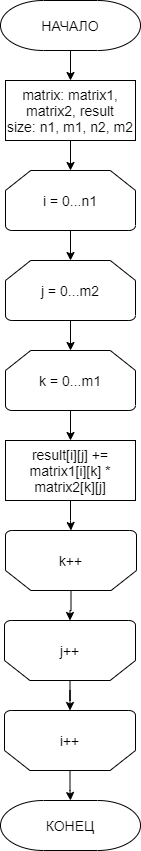
\includegraphics[width=0.12\linewidth]{base.jpg}
		\caption{Схема классического алгоритма умножения матриц}
		\label{fig:base}
	\end{figure}

	\newpage
	
	На рисунках \ref{fig:vin1}, \ref{fig:vin2}, \ref{fig:vin3}, \ref{fig:vin4} представлена схема алгоритма умножения матриц Винограда.
	
	\begin{figure}[h]
		\centering
		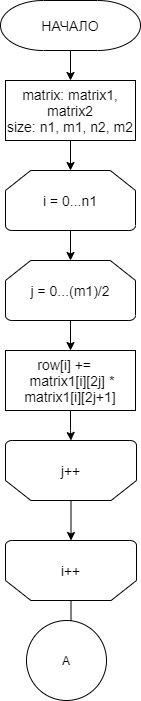
\includegraphics[width=0.202\linewidth]{vin1.jpg}
		\caption{Схема алгоритма Винограда (часть 1)}
		\label{fig:vin1}
	\end{figure}
	
	\newpage
	
	\begin{figure}[h]
		\centering
		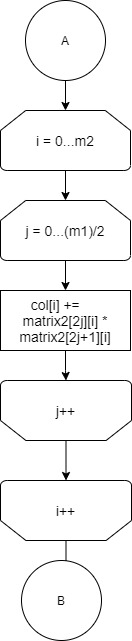
\includegraphics[width=0.207\linewidth]{vin2.jpg}
		\caption{Схема алгоритма Винограда (часть 2)}
		\label{fig:vin2}
	\end{figure}
	
	\newpage
	
	\begin{figure}[h]
		\centering
		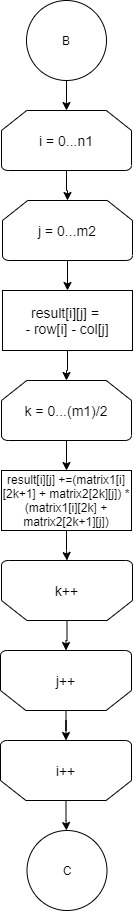
\includegraphics[width=0.146\linewidth]{vin3.jpg}
		\caption{Схема алгоритма Винограда (часть 3)}
		\label{fig:vin3}
	\end{figure}
	
	\newpage
	
	\begin{figure}[h]
		\centering
		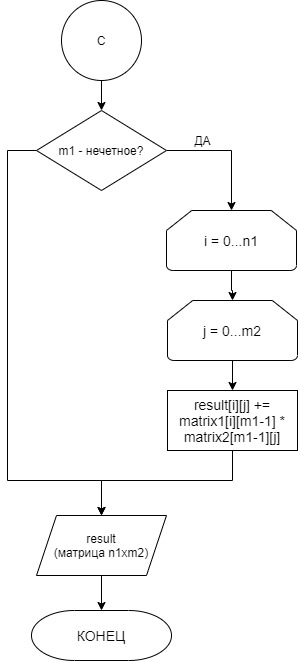
\includegraphics[width=0.4\linewidth]{vin4.jpg}
		\caption{Схема алгоритма Винограда (часть 4)}
		\label{fig:vin4}
	\end{figure}
	
	\newpage
	
	На рисунках \ref{fig:vinOpt1}, \ref{fig:vinOpt2}, \ref{fig:vinOpt3}, \ref{fig:vinOpt4} представлена схема оптимизированного алгоритма умножения матриц Винограда.
	
	\begin{figure}[h]
		\centering
		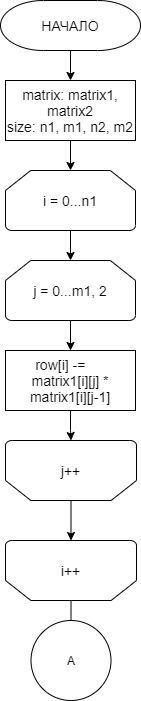
\includegraphics[width=0.202\linewidth]{vinopt1.jpg}
		\caption{Схема оптимизированного алгоритма Винограда(часть 1)}
		\label{fig:vinOpt1}
	\end{figure}
	
	\newpage
	
	\begin{figure}[h]
		\centering
		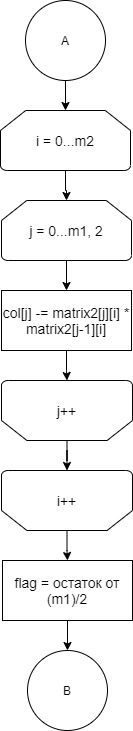
\includegraphics[width=0.18\linewidth]{vinopt2.jpg}
		\caption{Схема оптимизированного алгоритма Винограда(часть 2)}
		\label{fig:vinOpt2}
	\end{figure}
	
	\newpage
	
	\begin{figure}[h]
		\centering
		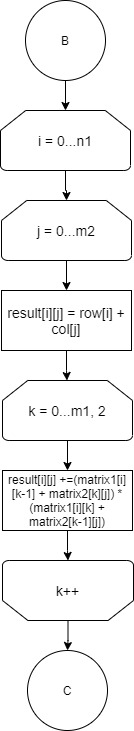
\includegraphics[width=0.18\linewidth]{vinopt3.jpg}
		\caption{Схема оптимизированного алгоритма Винограда(часть 3)}
		\label{fig:vinOpt3}
	\end{figure}
	
	\newpage 
	
	\begin{figure}[h]
		\centering
		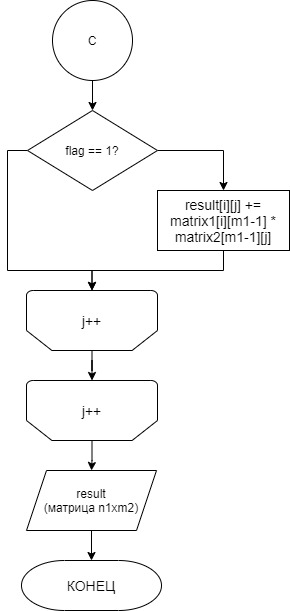
\includegraphics[width=0.4\linewidth]{vinopt4.jpg}
		\caption{Схема оптимизированного алгоритма Винограда(часть 4)}
		\label{fig:vinOpt4}
	\end{figure}
	
	\newpage
	
	\section{Оценка трудоемкости алгоритмов умножения матриц}
	\hfill
	\begin{enumerate}
		\item Стандартный алгоритм
		$$f=2+M(2+2+Q(2+2+N(2+8+1+1+1)))=13 \cdot$$
		
		$$\cdot MNQ+4MQ+4M+2 \approx 13 \cdot MNQ$$ 
		
		\item Алгоритм Винограда
		
		Трудоемкость алгоритма Винограда:\\
		
		Первый цикл: $\frac{15}{2} \cdot N  Q + 5 \cdot M + 2$ \\
		
		Второй цикл: $\frac{15}{2} \cdot M  N + 5 \cdot M + 2$\\
		
		Третий цикл: $13 \cdot M  N Q + 12 \cdot M Q + 4 \cdot M + 2$\\
		
		Условный переход: $\begin{bmatrix}
			2    &&, \text{лучший случай (при четном N)}\\
			15 \cdot QM + 4 \cdot M + 4 &&, \text{худший случай}\\
		\end{bmatrix} $ \\
		
		Итого: $f = \frac{15}{2} \cdot M  N + \frac{15}{2} \cdot Q  N + 9 \cdot M + 8 +  5 \cdot Q + 13 \cdot M  N Q + 12 \cdot M Q +
		\begin{bmatrix}
			2    &&, \text{в лучшем случае}\\
			15 \cdot QM + 4 \cdot M + 4 &&, \text{в худшем случае}\\
		\end{bmatrix} $ \\
		
		$$f \approx 13 \cdot MNQ $$
		
		\item Оптимизированный алгоритм Винограда
		
		Введем оптимизации: 
		\begin{enumerate}
			\item замена оперции = на += или -=
			\item избавление от деления в условиях цикла (j < N, j += 2)
			\item Заносим проверку на нечетность кол-ва строк внутрь основных циклов
			\item Расчет условия для последнего цикла один раз, а далее использование флага
		\end{enumerate}
		
		Первый цикл: $4 \cdot N  Q + 4 \cdot M + 2$ \\
		
		Второй цикл: $4 \cdot M  N + 4 \cdot M + 2$\\
		
		Третий цикл: $9 \cdot M  N Q + 10 \cdot M Q + 4 \cdot M + 2$\\
		
		Условный переход: $\begin{bmatrix}
			2   &&, \text{лучший случай (при четном N)}\\
			10 \cdot QM &&, \text{худший случай}\\
		\end{bmatrix} $ \\
		
		Трудоемкость оптимизированного алгоритма Винограда:\\
		
		Итого: $$f = 4 \cdot N  Q + 4 \cdot M + 2 + 4 \cdot M  N + 4 \cdot M + 2 + 9 \cdot M  N Q + 10 \cdot M Q + 4 \cdot M + 2 + $$
		
		$$ + \begin{bmatrix}
			2   &&, \text{л.c}\\
			10 \cdot QM &&, \text{х.c}\\
		\end{bmatrix} \approx 9 \cdot MNQ$$
		
		
	\end{enumerate}

	\section{Структуры данных}
	Для хранения матриц будут использоваться двумерные массивы. Для хранения предварительных вычислений в алгоритме Винограда - одномерные массивы.
	
	\section{Тестирование и классы эквивалентности}
	Для проверки работоспособности ПО будет применяться функциональное тестирование.
	
	Классы эквивалентности:
	
	\begin{itemize}
		\item квадратные матрицы одинаковых размеров;
		\item матрицы разных размеров (подходящие для умножения);
		\item в матрицах присутствуют как положительные, так и отрицательные числа;
		\item матрицы из одного элемента.
	\end{itemize}
	
	\section{Используемая память}
	Все используемые в данной работе массивы будут динамическими. В связи с этим, нужно будет контролировать проблемы с памятью, в частности при выделении памяти под массивы и её освобождении из-под них.
	
	Из всего вышесказанного следует, что количество памяти, необходимой алгоритмам, пропорционально размерам матриц.
	
	\section{Структура ПО}
	ПО будет состоять из набора функций:
	
	\begin{itemize}
		\item основная функция, работающая с меню;
		\item ввод исходных данных с клавиатуры;
		\item классический алгоритм умножения матриц;
		\item алгоритм Винограда;
		\item оптимизированный алгоритм Винограда;
		\item замеры времени.
	\end{itemize}
	
	\section{Вывод}
	На основе теоретических данных, полученные в аналитическом разделе были построены схемы иследуеммых  алгоритмов. Также были описаны: структуры данных, используемые в алгоритмах, способы тестирования и классы эквивалентности, память, используемая алгоритмом, и структура ПО.
	
	\chapter{Технологическая часть}
	
	В данном разделе будут разработаны исходные коды трех алгоритмов: классическое умножение матриц, алгоритм Винограда, оптимизированный алгоритм Винограда.
	
	\section{Средства реализации}
	Для реализации программы умножения двух матриц был выбран язык программирования Python. Данный выбор обусловлен тем,  что в этом языке присутсвует функция для измерения процессорного времени.
	
	\section{Реализация алгоритмов}
	
	В листингах \ref{std} - \ref{opt} приведена реализация алгоритмов умножения: стандартного, Винограда и Винограда с оптимизацией.
	
	\begin{lstlisting}[label=std,caption=Стандартный алгоритм умножения,language=Python]
	def std_mult(matr_a, matr_b, M, N, Q):
		res = [[0 for x in range(Q)] for y in range(M)]
			for i in range(M):
				for j in range(Q):
					for k in range(N):
						res[i][j] = res[i][j] + matr_a[i][k] * matr_b[k][j]
		return res
	\end{lstlisting}

	\newpage
	
	\begin{lstlisting}[label=win,caption=Алгоритм Винограда,language=Python]
	def precomp_rows(matr, M, N):
		mul_h = [0 for x in range(M)]
			for i in range(M):
				for j in range(0, N - 1, 2):
					mul_h[i] = mul_h[i] + matr[i][j] * matr[i][j + 1]
		return mul_h
	
	def precomp_cols(matr, M, N):
		mul_v = [0 for y in range(N)]
		for i in range(N):
			for j in range(0, M - 1, 2):
				mul_v[i] = mul_v[i] + matr[j][i] * matr[j + 1][i]
		return mul_v
	
	def win_mult(matr_a, matr_b, M, N, Q):
		res = [[0 for x in range(Q)] for y in range(M)]
	
		mul_h = precomp_rows(matr_a, M, N)
		mul_v = precomp_cols(matr_b, N, Q)
	
		for i in range(M):
			for j in range(Q):
				res[i][j] = -mul_h[i] - mul_v[j]
				for k in range(0, N - 1 , 2):
					res[i][j] = res[i][j] + (matr_a[i][k] + matr_b[k + 1][j]) * (matr_a[i][k + 1] + matr_b[k][j])
		if N % 2 != 0:
			for i in range(M):
				for j in range(Q):
					res[i][j] = res[i][j] + matr_a[i][N - 1] * matr_b[N - 1][j]
		return res
	\end{lstlisting}

	\newpage
	
	\begin{lstlisting}[label=opt,caption=Оптимизированный алгоритм Винограда,language=Python]
	def opt_precomp_rows(matr, M, N):
		mul_h = [0 for x in range(M)]
		for i in range(M):
			for j in range(0, N - 1, 2):
				mul_h[i] += (matr[i][j] * matr[i][j + 1])
		return mul_h
	
	def opt_precomp_cols(matr, M, N):
		mul_v = [0 for y in range(N)]
		for i in range(N):
			for j in range(0, M - 1, 2):
				mul_v[i] += (matr[j][i] * matr[j + 1][i])
		return mul_v
	
	def opt_win_mult(matr_a, matr_b, M, N, Q):
		res = [[0 for x in range(Q)] for y in range(M)]
	
		mul_h = opt_precomp_rows(matr_a, M, N)
		mul_v = opt_precomp_cols(matr_b, N, Q)
	
		odd = N % 2
	
		for i in range(M):
			for j in range(Q):
				res[i][j] = -mul_h[i] - mul_v[j]
				for k in range(0, N - 1 , 2):
					res[i][j] += ((matr_a[i][k] + matr_b[k + 1][j]) * (matr_a[i][k + 1] + matr_b[k][j]))
				if odd:
					res[i][j] += (matr_a[i][N - 1] * matr_b[N - 1][j])
		return res
	\end{lstlisting}
	
	\section{Тестовые данные}
	
	В таблице 3.1 приведены тестовые данные, на которых было протестированно разработанное ПО. Как видно из этой таблицы, все тесты были успешно пройдены, что означает, что программа работает правильно.
	
	\begin{table}[h]
		\label{tabular:functional_test}
		\begin{center}
			\begin{tabular}{ | c | c | c | c |}
				\hline
				\textbf{Первая матрица} & \textbf{Вторая матрица} & \textbf{Ожидаемый результат} & \textbf{Полученный результат}\\ \hline
				$\begin{bmatrix} 
					1&2&3 \\
					4&5&6 \\ 
					7&8&9 \\ 
				\end{bmatrix}$ & 
				$\begin{bmatrix} 
					1&2&3 \\
					4&5&6 \\ 
					7&8&9 \\ 
				\end{bmatrix}$ &
				$\begin{bmatrix} 
					30&36&42 \\
					66&81&96 \\ 
					102&126&150 \\ 
				\end{bmatrix}$ &
				$\begin{bmatrix} 
					30&36&42 \\
					66&81&96 \\ 
					102&126&150 \\ 
				\end{bmatrix} $\\ 
				\hline
				
				$\begin{bmatrix} 
					1&2 \\
					4&5 \\ 
					7&8 \\ 
				\end{bmatrix}$ & 
				$\begin{bmatrix} 
					1&2&3 \\
					4&5&6 \\ 
				\end{bmatrix}$ &
				$\begin{bmatrix} 
					9&12&15 \\
					24&33&42 \\ 
					39&54&69 \\ 
				\end{bmatrix} $ &
				$\begin{bmatrix} 
					9&12&15 \\
					24&33&42 \\ 
					39&54&69 \\ 
				\end{bmatrix} $ \\
				\hline
				
				$\begin{bmatrix} 
					8&-10&4 \\
					0&-7&6 \\ 
				\end{bmatrix}$ & 
				$\begin{bmatrix} 
					-7&1 \\
					-9&0 \\ 
					7&-3 \\ 
				\end{bmatrix}$ &
				$\begin{bmatrix} 
					62&-4 \\
					105&-18 \\  
				\end{bmatrix} $ &
				$\begin{bmatrix} 
					62&-4 \\
					105&-18 \\  
				\end{bmatrix} $ \\
				\hline
				
				$\begin{bmatrix} 
					10 \\ 
				\end{bmatrix}$ & 
				$\begin{bmatrix} 
					-5 \\ 
				\end{bmatrix}$ &
				$\begin{bmatrix} 
					-50 \\  
				\end{bmatrix} $ &
				$\begin{bmatrix} 
					-50 \\  
				\end{bmatrix} $ \\
				\hline
			\end{tabular}
		\end{center}
	\end{table} 

	\newpage
	
	\section{Вывод}
	В данном разделе были разработаны исходные коды трех алгоритмов: классическое умножение матриц, алгоритм Винограда, оптимизированный алгоритм Винограда, основная разница которого — наличие предварительной обработки, а также уменьшение количества операций умножения для увеличения эффективности.
	
	\chapter{Исследовательская часть}
	
	В этом разделе будет проведён эксперимент для определения эффективности по времени работы каждого из разработанных алгоритмов.
	
	\section{Пример работы}
	
	Демонстрация работы программы приведена на рисунке 4.1.
	
	\begin{figure}[h]
		\begin{center}
			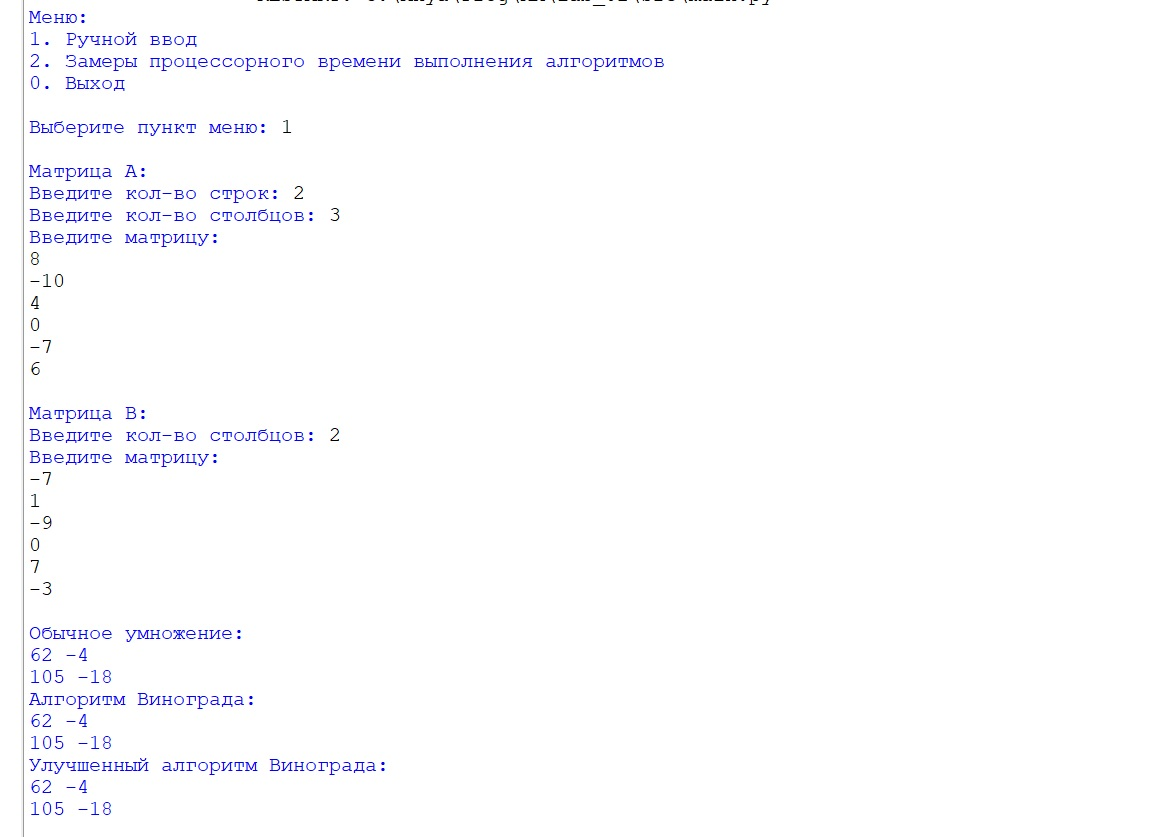
\includegraphics[scale=0.9]{example.jpg}
			\caption{Работа алгоритмов нахождения расстояния Левенштейна и Дамерау -- Левенштейна.}
		\end{center}
	\end{figure}
	
	\section{Технические характеристики}
	
	Ниже приведеные технические характеристики устройства, на котором было проведенно тестирование ПО:
	
	\begin{itemize}
		
		\item Операционная система: Windows 10 64-bit Home \cite{home}.
		
		\item Оперативная память: 8 GB.
		
		\item Процессор: 11th Gen Intel(R) Core(TM) i3-1115G4 @ 3.00GHz
		\cite{i3}.
		
	\end{itemize}
	
	\section{Время выполнения алгоритмов}
	Время выполнения алгоритмов замерялось с помощью функции process\_time модуля time в Python  \cite{process}. Данная функция возвращает значение в долях секунды суммы системного и пользовательского процессорного времени текущего процесса. \newline
	
	В таблицах 4.1 - 4.2 представлены замеры времени работы для каждого из алгоритмов.
	
	\begin{table} [h!]
		\caption{Лучший случай времени выполнения алгоритмов}
		\begin{center}
			\begin{tabular}{|c c c c|} 
				\hline
				Размер матриц & Стандартный & Виноград & Оптимизированный \\  
				\hline
				50 & 0.019375 & 0.017344 & 0.017344 \\
				\hline
				100 & 0.133750 & 0.125625 & 0.122813 \\
				\hline
				150 & 0.452813 & 0.411406 & 0.400313 \\
				\hline
				200 & 1.034063 & 0.937344 & 0.926719 \\
				\hline
				250 & 1.989219 & 1.825156 & 1.795313 \\
				\hline
			\end{tabular}
		\end{center}
	\end{table}

	\begin{table} [h!]
		\caption{Худший случай времени выполнения алгоритмов}
		\begin{center}
			\begin{tabular}{|c c c c|} 
				\hline
				Размер матриц & Стандартный & Виноград & Оптимизированный \\  
				\hline
				51 & 0.019062 & 0.018594 & 0.018281 \\
				\hline
				101 & 0.137031 & 0.127812 & 0.126719 \\
				\hline
				151 & 0.445937 & 0.410156 & 0.406875 \\
				\hline
				201 & 1.045000 & 0.958750 & 0.949375 \\
				\hline
				251 & 2.020000 & 1.839063 & 1.825469 \\
				\hline
			\end{tabular}
		\end{center}
	\end{table}
	
	\begin{figure}[h!]
		\begin{center}
			\begin{tikzpicture}
				\begin{axis}[
					legend pos = north west,
					xlabel=длина строки,
					ylabel=секунды,
					minor tick num = 1,
					grid = both,
					major grid style = {lightgray},
					minor grid style = {lightgray!25},
					xtick distance = 50,
					width = 0.9\textwidth,
					height = 0.5\textwidth]
					
					\addplot[
					blue,
					semithick,
					mark = x,
					mark size = 3pt,
					thick,
					] file {std.txt};
					
					\addplot[
					red,
					semithick,
					mark = *,
					] file {win.txt};
					
					\legend{
						Стандартный алгоритм,
						Алгоритм Винограда
					}
				\end{axis}
			\end{tikzpicture}
		\end{center}
		\caption{Сравнение стандартного алгоритма умножения и алгоритма Винограда}
	\end{figure}
	
	\begin{figure}[h!]
		\begin{center}
			\begin{tikzpicture}
				\begin{axis}[
					legend pos = north west,
					xlabel=длина строки,
					ylabel=секунды,
					minor tick num = 1,
					grid = both,
					major grid style = {lightgray},
					minor grid style = {lightgray!25},
					xtick distance = 50,
					width = 0.9\textwidth,
					height = 0.5\textwidth]
					
					\addplot[
					blue,
					semithick,
					mark = x,
					mark size = 3pt,
					thick,
					] file {win.txt};
					
					\addplot[
					red,
					semithick,
					mark = *,
					] file {opt.txt};
					
					\legend{
						Алгоритм Винограда,
						Оптимизированный алгоритм Винограда
					}
				\end{axis}
			\end{tikzpicture}
		\end{center}
		\caption{Сравнение алгоритма Винограда и оптимизированного алгоритма Винограда}
	\end{figure}

	\newpage
	
	\section{Вывод}
	
	В результате проведенного эксперимента можно сделать вывод, что алгоритм Винограда эффективнее стандартного алгоритма по времени в среднем примерно на 8,7\%.
	
	
	\chapter*{Заключение}
	\addcontentsline{toc}{chapter}{Заключение}
	
	В ходе проделанной работы были изучены и реализованы классический алгоритм умножения матриц, алгоритм Винограда и оптимизированный алгоритм Винограда. 
	
	Экспериментально было подтверждено различие по временной эффективности алгоритмов умножения матриц на материале замеров процессорного времени выполнения реализации на варьирующихся размерах матриц. Так, оптимизированный алгоритм Винограда работает чуть быстрее обычного алгоритма Винограда и зачительно быстрее классического алгоритма умножения матриц.
	
	На основании сравнения данных алгоритмов был сделан вывод, что алгоритм Винограда эффективнее классического алгоритма в среднем примерно на 8,7\%. При этом оптимизированный алгоритм Винограда сравним по времени с обычным алгоритмом Винограда.
	
	\addcontentsline{toc}{chapter}{Список литературы}
	
	\bibliographystyle{utf8gost705u}  % стилевой файл для оформления по ГОСТу
	
	\bibliography{biblio}          % имя библиографической базы (bib-файла)
	
\end{document}
